\documentclass[tikz,border=10pt]{standalone}
\usetikzlibrary{arrows.meta, positioning}

\begin{document}
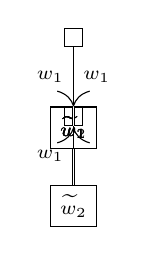
\begin{tikzpicture}[
  node distance=1cm and 0cm,
  every node/.style={font=\scriptsize},
  every rectangle node/.style={midway, auto=right},
  every arrow node label/.style={font=\scriptsize},
  >=Latex
]

\node (input) [draw] {};
\node (conv1) [right=of input, draw] {$\widetilde{w}_1$};
\node (pool1) [right=of conv1, draw] {};

\node (conv2a) [below=of pool1, draw] {$\widetilde{w}_2$};
\node (conv2b) [right=of conv2a, draw] {$\widetilde{w}_2$};
\node (conv2c) [right=of conv2b, draw] {$\widetilde{w}_1$};

\node (upconv1) [above=of conv2c, draw] {};
\node (conv3) [left=of upconv1, draw] {$\widetilde{w}_1$};

\node (output) [left=of conv3, draw] {};

\draw [double] (conv1) -- (pool1);
\draw (pool1) -- (conv2a) node [every arrow node label] {$w_1$};
\draw [double] (conv2a) -- (conv2b);
\draw [double] (conv2b) -- (conv2c);
\draw [dashed] (conv2c) -- (upconv1) node [every arrow node label] {$w_1$};
\draw [-{To[length=2mm]}] (upconv1) -- (conv3) node [every arrow node label] {$w_1$};
\draw [-{To[length=2mm]}] (conv3) -- (conv1);

\end{tikzpicture}
\end{document}